% \begin{table*}[!htbp]
%  \centering
%  \footnotesize
%  \caption{\textbf{Evaluation of various models on \benchmarkname.} We report the generalized accuracy of five types of evidence sources including pure text (TXT), layout (LAY), chart (CHA), table (TAB), and image (IMG). We also present the generalized accuracy of questions categorized by the number of evidence pages: single-page (SIN), cross-page (MUL), and unanswerable (UNA) questions. The \colorbox{firstBest}{\bf best} and \colorbox{secondBest}{\textbf{second-best}} performance in each section are highlighted.}
%  \label{tab:main_results}
%  \renewcommand\tabcolsep{2.5pt} % column space
%  \renewcommand\arraystretch{1.00} % row space
%  \resizebox{1.\linewidth}{!}{
%     \begin{tabular}{l cc|ccccc|ccc|cc}
%     \toprule
%      \multirow{2}{*}{\textbf{Model}} & \multirow{2}{*}{\textbf{\#Param}} & \textbf{Context} & \multicolumn{5}{c|}{\textbf{Evidence Source}} & \multicolumn{3}{c|}{\textbf{Evidence Page}} &  \multirow{2}{*}{\textbf{ACC}} & \multirow{2}{*}{\textbf{F1}} \\
%      &  & \textbf{Window} & \header{TXT} & \header{LAY} & \header{CHA} & \header{TAB} & \header{FIG} & SIN & MUL & UNA \\ 
%     \midrule
%     \multicolumn{13}{l}{\hfill \textit{OCR (Tesseract~\cite{smith2007overview}) + Large Language Models (LLMs)} } \\
%     \midrule
%     \textcolor{gray}{\textit{Open-source Models}} \\
%     ChatGLM-128k~\cite{bai2024longalign} & 6B & 128k & 23.4 & 12.7 & 9.7 & 10.2 & 12.2 & 18.8 & 11.5 & 18.1 & 16.3 & 14.9 \\
%     Mistral-Instruct-v0.2~\cite{jiang2023mistral} & 7B & 32k & 19.9 & 13.4 & 10.2 & 10.1 & 11.0 & 16.9 & 11.3 & 24.1 & 16.4 & 13.8 \\
%     Mixtral-Instruct-v0.1~\cite{jiang2024mixtral} & 8x7B & 32k & 24.2 & 14.8 & 12.5 & 15.0 & 13.7 & 21.3 & 14.1 & 13.1 & 17.0 & 16.9 \\
%     Mixtral-Instruct-v0.1~\cite{jiang2024mixtral} & 8x22B & 64k & 34.2 & 21.3 & 19.5 & 21.3 & 19.2 & 27.7 & 21.9 & 32.4 & 26.9 & 24.7 
%     \\
%     \textcolor{gray}{\textit{Proprietary Models}} \\
%     QWen-Plus~\cite{qwen1.5} & - & 32k & 17.4 & 15.6 & 7.4 & 7.9 & 8.8 & 14.2 & 10.6 & 42.2 & 18.9 & 13.4 \\
%     DeepSeek-V2~\cite{deepseekv2} & - & 32k & 27.8 & 19.6 & 8.8 & 17.0 & 9.4 & 20.2 & 15.4 & 48.1 & 24.9 & 19.6 \\
%     Claude-3 Opus~\cite{claude3} & - & 32k & 30.8 & 30.1 & 16.4 & 24.4 & 16.3 & 32.0 & 18.6 & 30.9 & 26.9 & 24.5 \\
%     Gemini-1.5-Pro~\cite{geminiteam2024gemini} & - & 32k & 29.3 & 15.9 & 12.5 & 17.7 & 11.5 & 21.2 & 16.4 & \colorbox{firstBest}{\textbf{73.4}} & 31.2 & 24.8 \\
%     GPT-4-turbo~\cite{openai2024gpt4} & - & 128k & 36.5 & 21.0 & 20.7 & 24.3 & 17.3 & 28.7 & 23.8 &  31.2 & 27.6 & 25.9 \\
%     GPT-4o~\cite{gpt4o} & - & 128k & \colorbox{secondBest}{41.1} & 23.4 & 28.5 & \colorbox{secondBest}{38.1} & 22.4 & 35.4 & 29.3 & 18.6 & 30.1 & 30.5 \\
%     \midrule
%     \multicolumn{13}{l}{\hfill \textit{Large Visual Language Models (LVLMs)}} \\
%     \midrule
%     \textcolor{gray}{\textit{Open-source, 7-14B Models}} \\
%     DeepSeek-VL-Chat~\cite{lu2024deepseek} & 7.3B & 4k & 7.2 & 6.5 & 1.6 & 5.2 & 7.6 & 5.2 & 7.0 & 12.8 & 7.4 & 5.4 \\
%     Idefics2~\cite{laurençon2024matters} & 8B & 8k & 9.0 & 10.6 & 4.8 & 4.1 & 8.7 & 7.7 & 7.2 & 5.0 & 7.0 & 6.8 \\
%     MiniCPM-Llama3-V2.5~\cite{yu2024rlaifv,xu2024llava-uhd} & 8B & 2k & 11.9 & 10.8 & 5.1 & 5.9 & 12.2 & 9.5 & 9.5 & 4.5 & 8.5 & 8.6 \\
%     % MiniCPM-Llama3-V2.6~\cite{yu2024rlaifv,xu2024llava-uhd} & 8B & 32k & 13.0 & 18.9 & 6.7 & 6.8 & 13.9 & 15.0 & 9.9 & 6.7 & 11.5 & 11.6 \\
%     InternLM-XC2-4KHD~\cite{dong2024internlm} & 8B & 16k & 9.9 & 14.3 & 7.7 & 6.3 & 13.0 & 12.6 & 7.6 & 9.6 & 10.3 & 9.8 \\
%     % InternLM-XC2d5~\cite{dong2024internlm} & 8B & 24k & 13.8 & 14.7 & 6.1 & 7.7 & 14.3 & 14.3 & 9.7 & 17.1 & 13.4 & 11.6 \\
%     mPLUG-DocOwl 1.5~\cite{hu2024mplug} & 8.1B & 4k & 8.2 & 8.4 & 2.0 & 3.4 & 9.9 & 7.4 & 6.4 & 6.2 & 6.9 & 6.3 \\
%     Qwen-VL-Chat~\cite{bai2023qwenvl} & 9.6B & 6k & 5.5 & 9.0 & 5.4 & 2.2 & 6.9 & 5.2 & 7.1 & 6.2 & 6.1 & 5.4 \\
%     % Qwen2-VL~\cite{bai2023qwenvl} & 8B & 32k & 33.2 & 29.4 & 20.1 & 22.3 & 30.8 & 35.9 & 20.9 & 13.5 & 26.1 & 26.9 \\
%     % Qwen2-VL~\cite{bai2023qwenvl} & 8B & 128k & 29.4 & 32.8 & 18.2 & 17.3 & 24.9 & 30.6 & 18.3 & 7.0 & 21.3 & 22.7 \\
%     % Monkey-Chat~\cite{li2023monkey} & 9.8B & 2k & 6.8 & 7.2 & 3.6 & 6.7 & 9.4 & 6.6 & 6.2 & 6.2 & 6.2 & 5.6 \\
%     \textcolor{gray}{\textit{Open-source, >14B Models}} \\
%     % Aria~\cite{li2024ariaopenmultimodalnative} & 8x3.5B & 64k & 29.1 & 24.0 & 15.5 & 24.4 & 20.4 & 31.3 & 18.3 & 38.1 & 28.3 & 24.6 \\
%     CogVLM2-LLaMA3-Chat~\cite{wang2023cogvlm} & 19B & 8k & 3.7 & 2.7 & 6.0 & 3.2 & 6.9 & 3.9 & 5.3 & 3.7 & 4.4 & 4.0 \\
%     InternVL-Chat-v1.5~\cite{chen2024far} & 26B & 4k & 14.0 & 16.2 & 7.1 & 10.1 & 16.6 & 14.9 & 12.2 & 17.5 & 14.6 & 13.0 \\
%     EMU2-Chat~\cite{} & 37B & 2k & 6.1 & 9.7 & 2.6 & 3.8 & 7.7& 5.7 &6.1 &16.5& 8.3& 5.5
%     % InternVL-Chat-v2~\cite{chen2024far} & 40B & 8k & 17.9 & 22.6 & 13.2 & 12.9 & 23.8 & 22.6 & 15.2 & 12.9 & 18.2 & 17.9 \\
%     % Qwen2-VL~\cite{bai2023qwenvl} & 72B & 128k & 39.7 & \colorbox{secondBest}{39.4} & \colorbox{secondBest}{36.4} & 34.3 & \colorbox{secondBest}{37.8} & \colorbox{secondBest}{46.2} & \colorbox{secondBest}{30.5} & 8.5 & \colorbox{secondBest}{33.3} & \colorbox{secondBest}{35.7} \\
%     % EMU2-Chat~\cite{sun2023generative} & 37B & 2k & 6.1 & 9.7 & 2.6 & 3.8 & 7.7 & 5.7 & 6.1 & 16.5 & 8.3 & 5.5 \\
%     \textcolor{gray}{\textit{Proprietary Models}} \\
%     Claude-3 Opus~\cite{claude3} & - & 200k & 24.9 & 24.7 & 14.8 & 13.0 & 17.1 & 25.6 & 13.8  & 7.6 & 17.4 & 18.1 \\
%     Gemini-1.5-Pro~\cite{geminiteam2024gemini} & - & 128k & 21.0 & 17.6 & 6.9 & 14.5 & 15.2 & 21.1 & 11.1 &  \colorbox{secondBest}{69.2} & 28.2 & 20.6 \\
%     GPT-4V(ision)~\cite{openai2024gpt4} & - & 128k & 34.4 & 28.3 & 28.2 & 32.4 & 26.8 & 36.4 & 27.0 & 31.2 & 32.4 & 31.2 \\
%     % GPT-4o-mini~\cite{gpt4o} & - & 128k & 29.4 & 28.5 & 19.9 & 37.3 & 25.2 & 36.8 & 22.2 & 22.0 & 29.0 & 28.6 \\
%     GPT-4o~\cite{gpt4o} & - & 128k & \colorbox{firstBest}{\textbf{46.3}} & \colorbox{firstBest}{\textbf{46.0}} & \colorbox{firstBest}{\textbf{45.3}} & \colorbox{firstBest}{\textbf{50.0}} & \colorbox{firstBest}{\textbf{44.1}} & \colorbox{firstBest}{\textbf{54.5}} & \colorbox{firstBest}{\textbf{41.5}} & 20.2 & \colorbox{firstBest}{\textbf{42.8}} & \colorbox{firstBest}{\textbf{44.9}} \\
%     \midrule
%     \multicolumn{13}{l}{\hfill \textit{Human Baseline}} \\
%     \midrule
%     Human Experts & - & -  & - & -  & -  & -  & -  &-  & -  & - & 65.8 & 66.0 \\
%     \bottomrule
%     \end{tabular}
%     }
% \end{table*}


\begin{table*}[!htbp]
 \centering
 \footnotesize
 \caption{\textbf{Evaluation of various models on \benchmarkname.} We report the generalized accuracy of five types of evidence sources including pure text (TXT), layout (LAY), chart (CHA), table (TAB), and image (IMG). We also present the generalized accuracy of questions categorized by the number of evidence pages: single-page (SIN), cross-page (MUL), and unanswerable (UNA) questions. The \colorbox{firstBest}{\bf best} and \colorbox{secondBest}{\textbf{second-best}} performance in each section are highlighted.}
 \label{tab:main_results}
 \renewcommand\tabcolsep{2.5pt} % column space
 \renewcommand\arraystretch{1.00} % row space
 \resizebox{0.95\linewidth}{!}{
    \begin{tabular}{l cc|ccccc|ccc|cc}
    \toprule
     \multirow{2}{*}{\textbf{Model}} & \multirow{2}{*}{\textbf{\#Param}} & \textbf{Context} & \multicolumn{5}{c|}{\textbf{Evidence Source}} & \multicolumn{3}{c|}{\textbf{Evidence Page}} &  \multirow{2}{*}{\textbf{ACC}} & \multirow{2}{*}{\textbf{F1}} \\
     &  & \textbf{Window} & \header{TXT} & \header{LAY} & \header{CHA} & \header{TAB} & \header{FIG} & SIN & MUL & UNA \\ 
    \midrule
    \multicolumn{13}{l}{\hfill \textit{OCR (Tesseract~\cite{smith2007overview}) + Large Language Models (LLMs)} } \\
    \midrule
    \textcolor{gray}{\textit{Open-source Models}} \\
    ChatGLM-128k~\cite{bai2024longalign} & 6B & 128k & 23.4 & 12.7 & 9.7 & 10.2 & 12.2 & 18.8 & 11.5 & 18.1 & 16.3 & 14.9 \\
    Mistral-Instruct-v0.2~\cite{jiang2023mistral} & 7B & 32k & 19.9 & 13.4 & 10.2 & 10.1 & 11.0 & 16.9 & 11.3 & 24.1 & 16.4 & 13.8 \\
    Mixtral-Instruct-v0.1~\cite{jiang2024mixtral} & 8x7B & 32k & 24.2 & 14.8 & 12.5 & 15.0 & 13.7 & 21.3 & 14.1 & 13.1 & 17.0 & 16.9 \\
    Mixtral-Instruct-v0.1~\cite{jiang2024mixtral} & 8x22B & 64k & 34.2 & 21.3 & 19.5 & 21.3 & 19.2 & 27.7 & 21.9 & 32.4 & 26.9 & 24.7 
    \\
    \textcolor{gray}{\textit{Proprietary Models}} \\
    QWen-Plus~\cite{qwen1.5} & - & 32k & 17.4 & 15.6 & 7.4 & 7.9 & 8.8 & 14.2 & 10.6 & 42.2 & 18.9 & 13.4 \\
    DeepSeek-V2~\cite{deepseekv2} & - & 32k & 27.8 & 19.6 & 8.8 & 17.0 & 9.4 & 20.2 & 15.4 & 48.1 & 24.9 & 19.6 \\
    Claude-3 Opus~\cite{claude3} & - & 32k & 30.8 & \colorbox{secondBest}{30.1} & 16.4 & 24.4 & 16.3 & 32.0 & 18.6 & 30.9 & 26.9 & 24.5 \\
    Gemini-1.5-Pro~\cite{geminiteam2024gemini} & - & 32k & 29.3 & 15.9 & 12.5 & 17.7 & 11.5 & 21.2 & 16.4 & \colorbox{firstBest}{\textbf{73.4}} & 31.2 & 24.8 \\
    GPT-4-turbo~\cite{openai2024gpt4} & - & 128k & 36.5 & 21.0 & 20.7 & 24.3 & 17.3 & 28.7 & 23.8 &  31.2 & 27.6 & 25.9 \\
    GPT-4o~\cite{gpt4o} & - & 128k & \colorbox{secondBest}{41.1} & 23.4 & \colorbox{secondBest}{28.5} & \colorbox{secondBest}{38.1} & 22.4 & 35.4 & \colorbox{secondBest}{29.3} & 18.6 & 30.1 & 30.5 \\
    \midrule
    \multicolumn{13}{l}{\hfill \textit{Large Visual Language Models (LVLMs)}} \\
    \midrule
    \textcolor{gray}{\textit{Open-source, 7-14B Models}} \\
    DeepSeek-VL-Chat~\cite{lu2024deepseek} & 7.3B & 4k & 7.2 & 6.5 & 1.6 & 5.2 & 7.6 & 5.2 & 7.0 & 12.8 & 7.4 & 5.4 \\
    Idefics2~\cite{laurençon2024matters} & 8B & 8k & 9.0 & 10.6 & 4.8 & 4.1 & 8.7 & 7.7 & 7.2 & 5.0 & 7.0 & 6.8 \\
    MiniCPM-Llama3-V2.5~\cite{yu2024rlaifv,xu2024llava-uhd} & 8B & 2k & 11.9 & 10.8 & 5.1 & 5.9 & 12.2 & 9.5 & 9.5 & 4.5 & 8.5 & 8.6 \\
    InternLM-XC2-4KHD~\cite{dong2024internlm} & 8B & 16k & 9.9 & 14.3 & 7.7 & 6.3 & 13.0 & 12.6 & 7.6 & 9.6 & 10.3 & 9.8 \\
    mPLUG-DocOwl 1.5~\cite{hu2024mplug} & 8.1B & 4k & 8.2 & 8.4 & 2.0 & 3.4 & 9.9 & 7.4 & 6.4 & 6.2 & 6.9 & 6.3 \\
    Qwen-VL-Chat~\cite{bai2023qwenvl} & 9.6B & 6k & 5.5 & 9.0 & 5.4 & 2.2 & 6.9 & 5.2 & 7.1 & 6.2 & 6.1 & 5.4 \\
    Monkey-Chat~\cite{li2023monkey} & 9.8B & 2k & 6.8 & 7.2 & 3.6 & 6.7 & 9.4 & 6.6 & 6.2 & 6.2 & 6.2 & 5.6 \\
    \textcolor{gray}{\textit{Open-source, >14B Models}} \\
    CogVLM2-LLaMA3-Chat~\cite{wang2023cogvlm} & 19B & 8k & 3.7 & 2.7 & 6.0 & 3.2 & 6.9 & 3.9 & 5.3 & 3.7 & 4.4 & 4.0 \\
    InternVL-Chat-v1.5~\cite{chen2024far} & 26B & 4k & 14.0 & 16.2 & 7.1 & 10.1 & 16.6 & 14.9 & 12.2 & 17.5 & 14.6 & 13.0 \\
    EMU2-Chat~\cite{sun2023generative} & 37B & 2k & 6.1 & 9.7 & 2.6 & 3.8 & 7.7 & 5.7 & 6.1 & 16.5 & 8.3 & 5.5 \\
    \textcolor{gray}{\textit{Proprietary Models}} \\
    Claude-3 Opus~\cite{claude3} & - & 200k & 24.9 & 24.7 & 14.8 & 13.0 & 17.1 & 25.6 & 13.8  & 7.6 & 17.4 & 18.1 \\
    Gemini-1.5-Pro~\cite{geminiteam2024gemini} & - & 128k & 21.0 & 17.6 & 6.9 & 14.5 & 15.2 & 21.1 & 11.1 &  \colorbox{secondBest}{69.2} & 28.2 & 20.6 \\
    GPT-4V(ision)~\cite{openai2024gpt4} & - & 128k & 34.4 & 28.3 & 28.2 & 32.4 & \colorbox{secondBest}{26.8} & \colorbox{secondBest}{36.4} & 27.0 & 31.2 & \colorbox{secondBest}{32.4} & \colorbox{secondBest}{31.2} \\
    GPT-4o~\cite{gpt4o} & - & 128k & \colorbox{firstBest}{\textbf{46.3}} & \colorbox{firstBest}{\textbf{46.0}} & \colorbox{firstBest}{\textbf{45.3}} & \colorbox{firstBest}{\textbf{50.0}} & \colorbox{firstBest}{\textbf{44.1}} & \colorbox{firstBest}{\textbf{54.5}} & \colorbox{firstBest}{\textbf{41.5}} & 20.2 & \colorbox{firstBest}{\textbf{42.8}} & \colorbox{firstBest}{\textbf{44.9}} \\
    \bottomrule
    \multicolumn{13}{l}{\hfill \textit{Human Baseline}} \\
    \midrule
    Human Experts & - & -  & - & -  & -  & -  & -  &-  & -  & - & 65.8 & 66.0 \\
    \bottomrule
    \end{tabular}
    }
\end{table*}

\section{Evaluation}\label{sec:evaluation}

\subsection{Evaluation Protocol}
We follow MATHVISTA~\cite{lu2024mathvista} to conduct a three-step evaluation protocol: \textit{response generation}, \textit{answer extraction}, and \textit{score calculation}. We adopt such a protocol out of three considerations: (1) Current LVLMs are instructed to generate long responses, rather than short-form answers, in conventional settings. (2) The evaluation of long responses, however, remains an open and challenging problem. (3) We focus on the document understanding (not instruction following) abilities of LVLMs.

Specifically, we impose no limitations on \textit{response generation} stage to encourage LVLMs to answer the questions in a freestyle. Then we propose a unified LLM-based \textit{answer extractor} (GPT-4o under our setting) to convert their long responses to short-form answers. Finally, we use a rule-based \textit{score calculator} to evaluate the converted short answers. We report both generalized accuracy and generalized F1 score to balance the answerable (positive) and unanswerable (negative) questions. The used prompt, the high correlation between our automatic \textit{answer extractor} and human evaluation, and the detailed rules of our \textit{score calculation} are described in Appendix~\ref{appendix: experimental_details}.


\subsection{Experimental Setup}
We evaluate 14 LVLMs on \benchmarkname, including 4 proprietary LVLMs and 10 open-source LVLMs. To purely evaluate LVLMs' long-context DU abilities, we screenshot each page of the PDF-formatted document with 144 DPI and feed all these PNG-formatted images to LVLMs in an end-to-end approach. Notably, all evaluated open-source LVLMs do not support multi-image inputs or present significant performance drops when fed with excessive images (\eg more than 10 or 20 images). Therefore, we employ a concatenation strategy that combines all screenshot pages into 1 or 5 images and feeds these concatenated images to open-source LVLMs. Regarding proprietary LVLMs, we adopt the same concatenation strategy and reduce the image number to 20 for Claude-3-Opus to fit its maximum image threshold. For GPT-4o, GPT-4V, and Gemini-1.5-Pro, we directly send all original screenshots to them (\ie the image number equals the page number).

For comparison, we also use the Tesseract~\cite{smith2007overview} OCR model to recognize and extract texts from the documents and feed the parsed documents to 10 LLMs, including 6 proprietary and 4 open-source ones. Texts exceeding their context lengths are truncated. Notably, as a key component of the classical solution for the DU task, the OCR model can handle most flattened texts and some structured tables in the document. However, it cannot perceive the information from the charts or images. Thus the TXT-formatted, OCR-parsed documents are lossy documents in which the information is not fully preserved. More detailed hyperparameters are introduced in Appendix~\ref{appendix: Hyperparameters}. Additionally, we also conduct manual evaluation on a subset of our datasets (238 questions from 29 documents) to indicate the difficulty of this task for humans.

\subsection{Main Results}
We compare the performance of different LVLMs and LLMs in Table~\ref{tab:main_results}, reporting their generalized accuracy and F1 scores (shown in the last two columns). Regarding LVLMs, we draw several conclusions as below: (1) The performance demonstrates that long-context DU is still a challenging and unsolved task for current LVLMs. The best-performing LVLM, GPT-4o, merely achieves a 44.9\% F1 score. The second best-performing LVLM, GPT-4V, lags behind by over 10\% percent and presents a 31.4\% F1 score. All other LVLMs only achieve about 20\% or even lower F1 scores. (2) Though far from satisfactory, GPT-4o performs much better than all other models (including GPT-4V). Thus we speculate that the multi-modal pre-training paradigm significantly benefits LVLMs' cross-modality understanding capabilities. (3) Proprietary LVLMs perform better than open-source LVLMs by a large margin. We attribute it to the difference of acceptable image numbers: open-source LVLMs only support single-image or several-image
% ~\footnote{We observe that all open-source LVLMs struggle when fed with more than 5 images.} 
inputs, while proprietary LVLMs can be fed with at least 20 images or even more. Given that lengthy documents have tens of even hundreds of pages, it is impractical for open-source LVLMs to accurately perceive the information in the documents from the excessively concatenated images. (4) The performances of different models are highly correlated with their acceptable image numbers and maximum image resolutions. Notably, open-source LVLMs that support high-resolution images (\ie InternLM-XC2-4KHD and InternVL-Chat-v1.5) exhibit superior performance compared to those with lower resolution limits.

Surprisingly, LVLMs even demonstrate overall worse performance than LLMs, even LLMs are fed with lossy OCR-parsed documents. Specifically, Gemini-1.5-Pro and Claude-3 Opus have 4.2\% and 6.4\% absolute F1-score degradations on vision versions. And the best-performing LLM (Mixtral) also surpasses the best-performing LVLM (InternVL-v1.5) by 11.7\%. The above results clearly reveal that most current LVLMs are still not proficient in cross-modality, long-context document understandings. It is promising that GPT-4o and GPT-4-turbo achieve better performance when seeing multi-modality PDF documents than parsed text by 14.4\% and 5.3\% F1-score, respectively. Their performances validate the feasibility, benefit, and necessity of understanding documents in an end-to-end, cross-modality approach. We speculate that the scarce related pre-training corpus (\ie extremely multi-image or lengthy documents) hinders the long-context DU capabilities of other LVLMs. We will leave related explorations for future work.

Regarding the human evaluation, we observe 66.0\% F1-score from our annotators and a significant performance gap (exceeding 20\% in absolute) between the current LVLMs and humans. This gap highlights the challenges of document understanding for LVLMs and the necessity of our benchmark.

\subsection{Fine-grained Results.} 

\begin{figure}
    \centering
    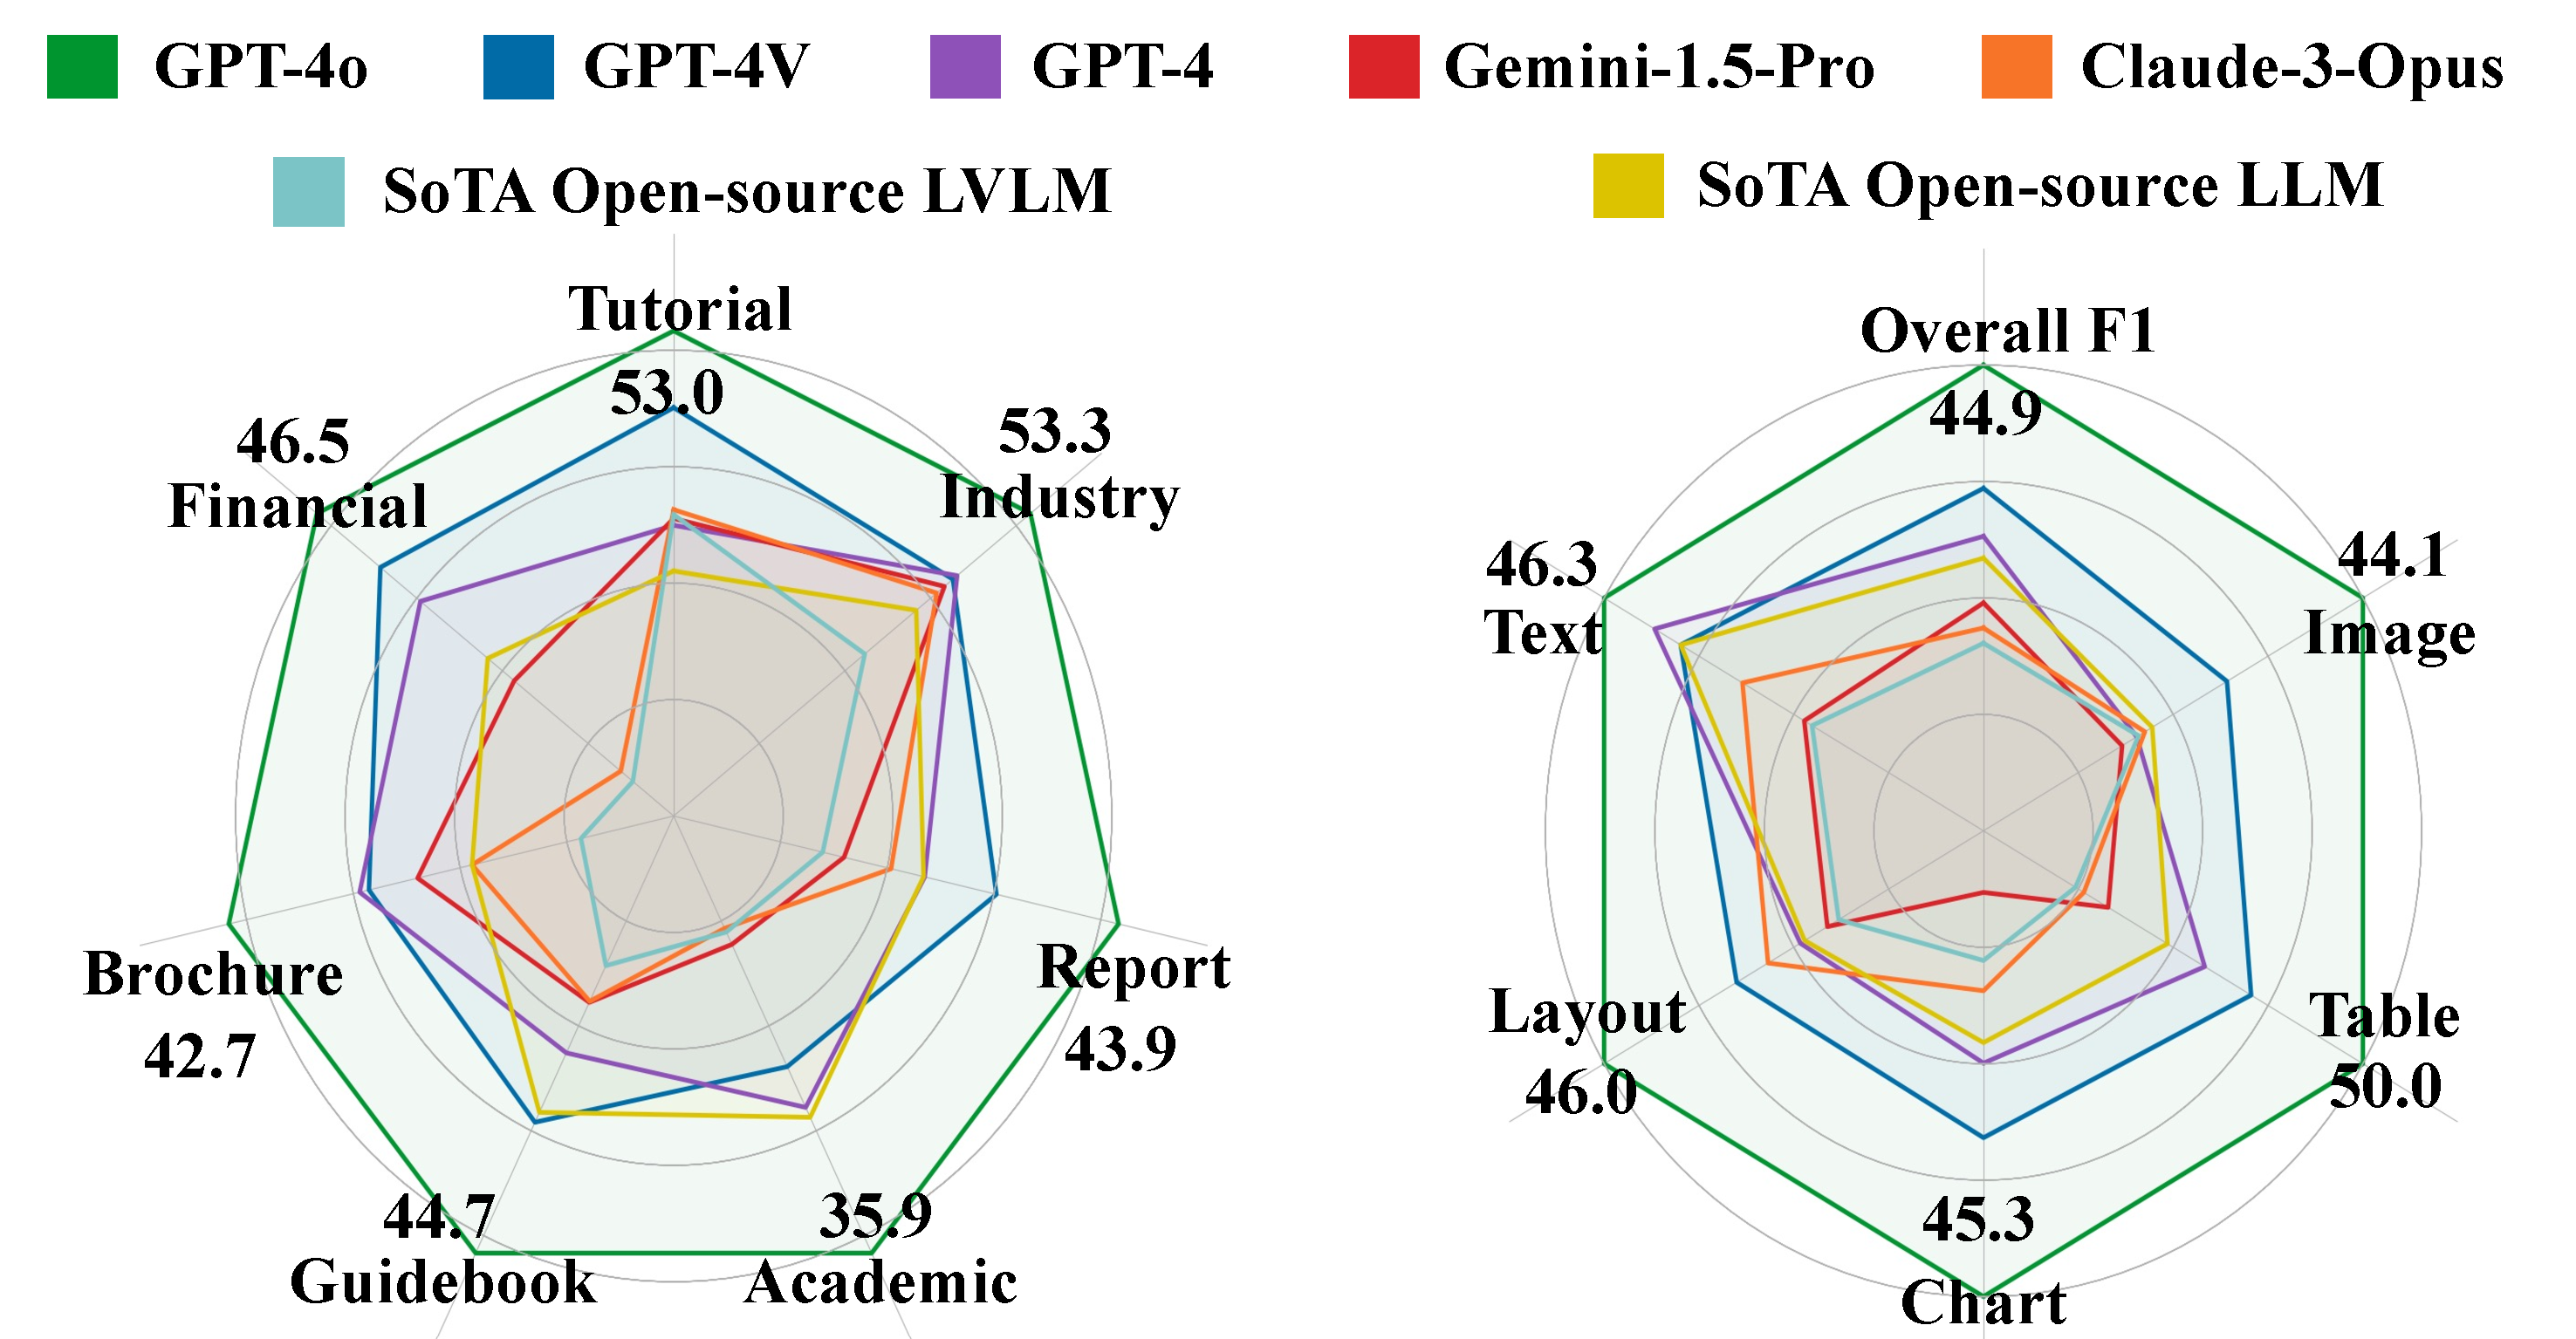
\includegraphics[width=0.8\textwidth]{figures/Radar.pdf}
    \caption{Fine-grained results on various document types and evidence sources.}
    \label{fig: radar_plot}
\end{figure}

\noindent{\textbf{Document Type.}} As illustrated in Figure~\ref{fig: radar_plot}, LVLMs and LLMs exhibit distinct performance patterns across various document types. Our findings include: (1) All evaluated models demonstrate decent performance on industrial documents, which tend to have more standardized formats and less non-textual information. (2) The GPT series and Mixtral (\ie the SoTA open-source LLM) show relatively balanced performance across different document types. In contrast, other models perform significantly worse in specialized domains such as academic papers and financial reports. (3) When equipped with OCR, LLM-based models like GPT-4 and Mixtral achieve comparable or even superior performance on industrial documents, academic papers, and brochures. Conversely, end-to-end LVLMs outperform OCR+LLMs in areas such as tutorials, research reports, and guidelines. We speculate that comprehending these latter document types requires more extensive multi-modal information, from which LVLMs significantly benefit.

\noindent{\textbf{Evidence Source.}} 
We categorize questions based on their evidence sources and present fine-grained results in Figure~\ref{fig: radar_plot} and Table~\ref{tab:main_results}. Our observations reveal that only GPT-4o exhibits relatively balanced performance across the different sources. Other LVLMs, however, show inferior performance on questions related to charts and/or images compared to those related to text and/or layout. Additionally, LLMs generally demonstrate better or comparable performance to LVLMs on text- and table-related questions but show worse performance on questions involving other elements. This highlights the limitations of OCR (and other PDF parsers) when dealing with charts and images, as well as the gap in OCR capabilities between LVLMs and pure-text LLMs.

\begin{wrapfigure}{r}{0.42\textwidth}
    % \vspace{-20pt}
    \centering
    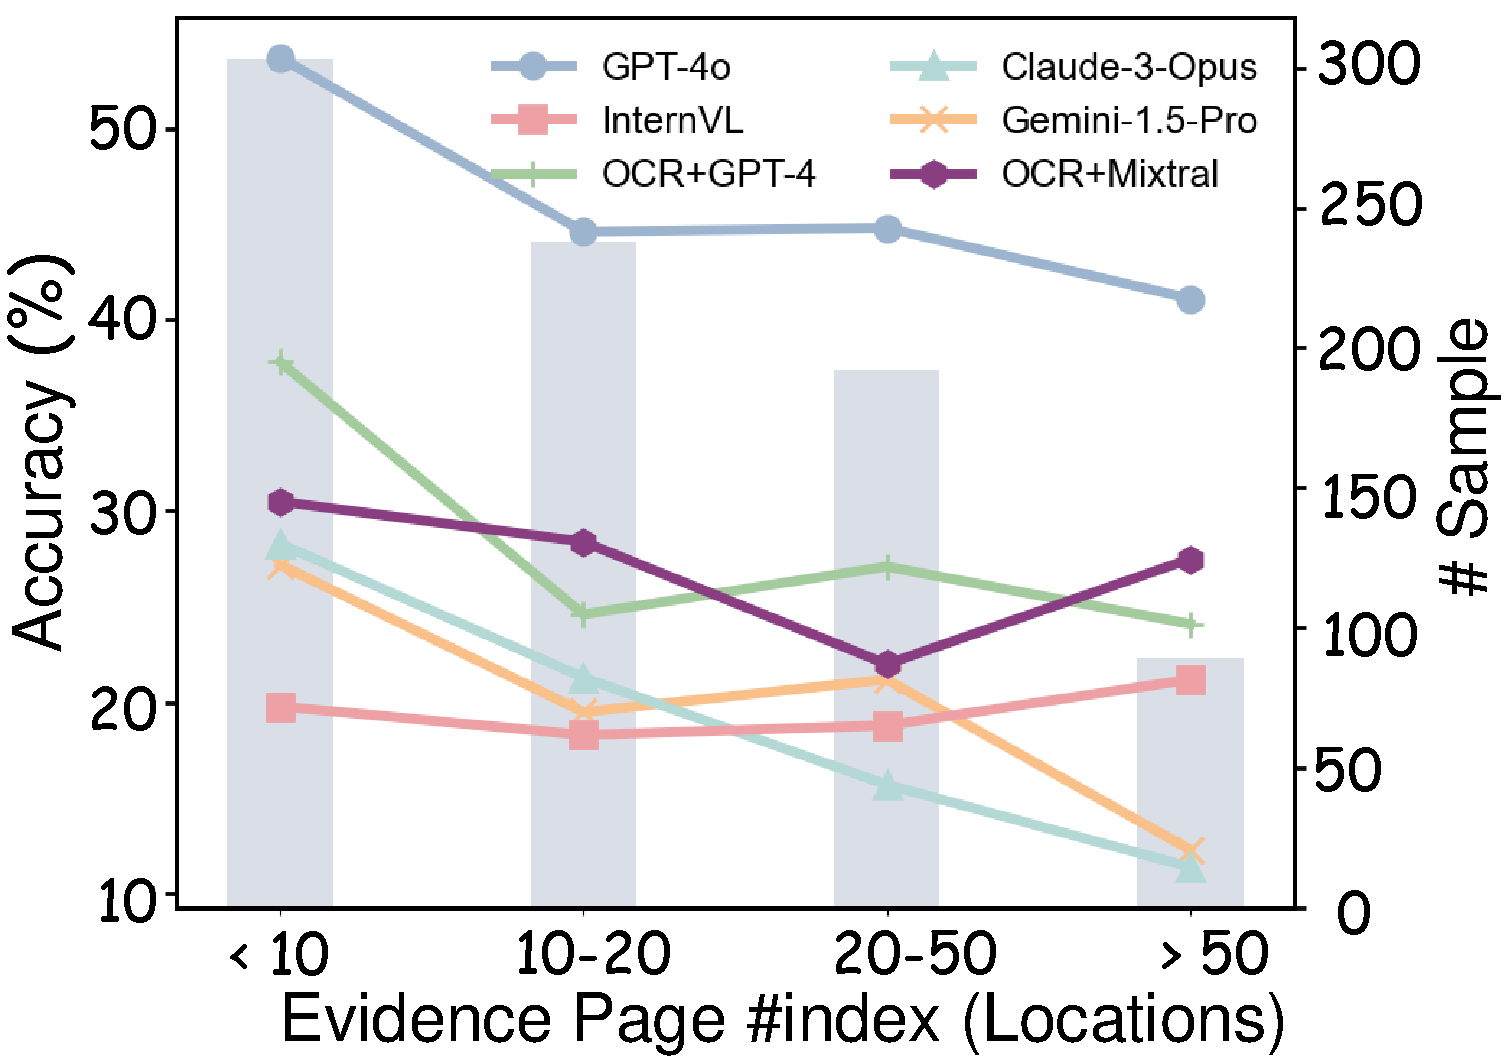
\includegraphics[width=\linewidth, bb=0 0 680 496]{figures/evidence_location_revised.pdf}
    \caption{Relationships between evidence positions and model performances.}
    \label{fig:evidence_page}
    % \vspace{-10pt}
\end{wrapfigure}

\noindent{\textbf{Evidence Position.}}
We also examine how the evidence locations (\ie the page indexes where the answer evidence is found) affect model performance. The results shown in Figure~\ref{fig:evidence_page} reinforce that \benchmarkname poses significant challenges for current models, at least partially due to the extended length of the documents. Almost all models (except InternVL-v1.5) exhibit their best performance on questions derived from the initial pages, while their performance declines progressively as the page index increases. Interestingly, two proprietary models, Gemini-Pro-1.5 and Claude-3-Opus, experience particularly sharp declines in performance.

\noindent{\textbf{Number of Evidence Page.}} 
We observe a consistent trend that all models achieve higher scores on single-page questions than cross-page questions. It reveals that gathering and reasoning over all necessary information across different pages is not trivial for current LVLMs and LLMs. More interestingly, evaluated LVLMs behave differently on unanswerable questions. GPT-4o and Claude-3 Opus adopt more aggressive strategies and usually tend to provide some answers. It makes their answers more likely helpful, but also increases the risk of hallucination and unfaithfulness (see their scores on unanswerable questions are much lower than answerable questions). On the contrary, Gemini-1.5-Pro, DeepSeek-VL-Chat, and EMU2-Chat are much more cautious and tend to refuse to answer questions about which they are uncertain. It makes their answers safer but less helpful (with large amounts of responses like \textit{I don't know}).